\subsection{\texorpdfstring{Control plots for $\tauTau$ channel}{Control plots for tau-tau channel}}
In this section, some control plots in $\tauTau$ channel are presented. In the left plot of figure~\ref{fig:met_mindphi}, the distribution of \MET at pre-selection before cutting on this variable is shown. The right plot of the same figure shows the distribution of the $\mindphifour$ variable at pre-selection before cutting on this variable.
\begin{figure}[!Hhtb]
\centering
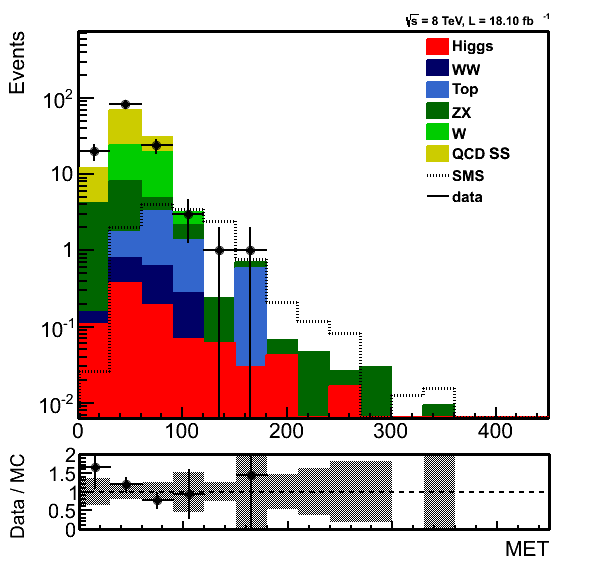
\includegraphics[angle=0,scale=0.35]{TauTauFigs/MET2.png}
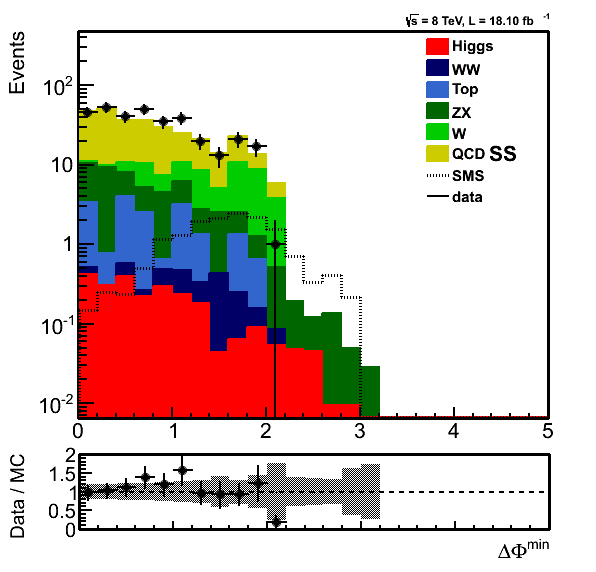
\includegraphics[angle=0,scale=0.35]{TauTauFigs/DPhimin.png} \\
\caption{The distributions of \MET (left) and $\mindphifour$ (right) at pre-selection. For each plot the cut on that variable is relaxed.}
\label{fig:met_mindphi}
\end{figure}

The jet multiplicity plot (jets with $\pt>40\GeV$ and $|\eta|<5$) for those jets which contribute to the $\mindphifour$ quantity is shown in the plots of figure~\ref{fig:njetsformindphi}. The left (right) plot is made at pre-selection with $\mindphifour$ relaxed (applied).
\begin{figure}[!Hhtb]
\centering
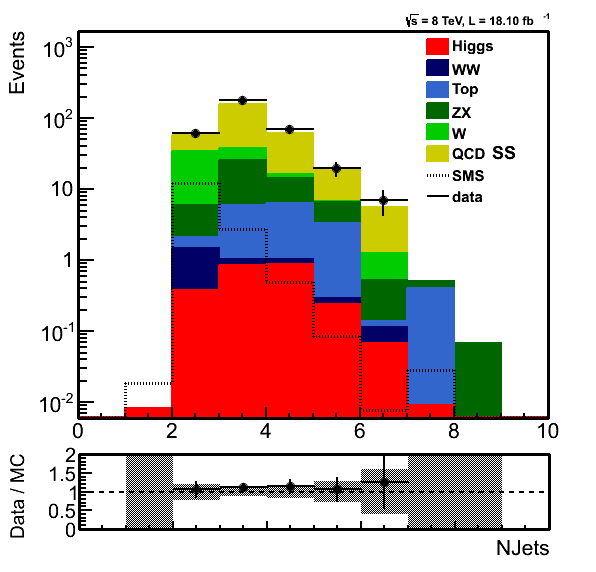
\includegraphics[angle=0,scale=0.35]{TauTauFigs/NJets_MinDphirelaxed.png}
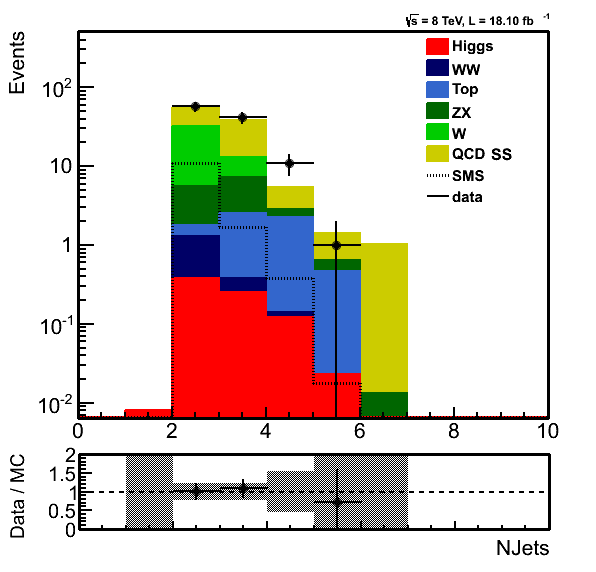
\includegraphics[angle=0,scale=0.35]{TauTauFigs/NJets.png} \\
\caption{The jet multiplicity distributions which enter the $\mindphifour$ quantity at pre-selection. Left (Right): $\mindphifour$ relaxed (applied).}
\label{fig:njetsformindphi}
\end{figure}

Figure~\ref{fig:ditaumass} contains the distributions of $m_{\tau\tau}$ at pre-selection with Z-veto cut is relaxed. For the right plot, the cut on $\mttwo>40\GeV$} is also relaxed.
\begin{figure}[!Hhtb]
\centering
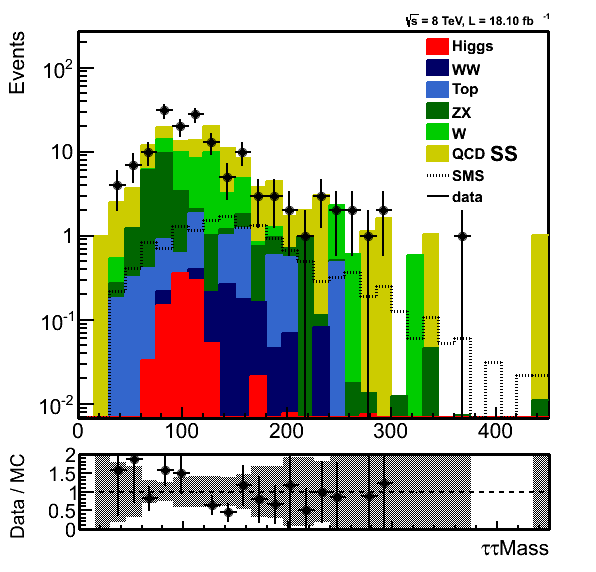
\includegraphics[angle=0,scale=0.35]{TauTauFigs/Invmass.png}
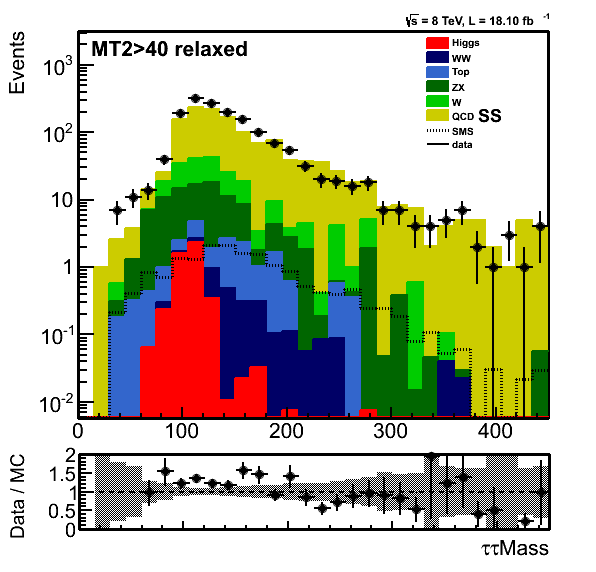
\includegraphics[angle=0,scale=0.35]{TauTauFigs/InvmassMT2relaxed.png} \\
\caption{The distributions of $m_{\tau\tau}$ at pre-selection. For both plots the Z-veto cut is relaxed. The cut on $\mttwo>40\GeV$ is also relaxed for the right plot.}
\label{fig:ditaumass}
\end{figure}


For all of the above plots, QCD shape and normalization is taken from data in SS events. Also the SMS point which is shown corresponds to (240,40).

The left (right) plot in figure~\ref{fig:nbjets} is the multiplicity of the bjets tagged by CSVM algorithm in the \binone (\bintwo). It is obvious that vetoing bjets in \bintwo would help to suppress background events from ttbar. 

\begin{figure}[!Hhtb]
\centering
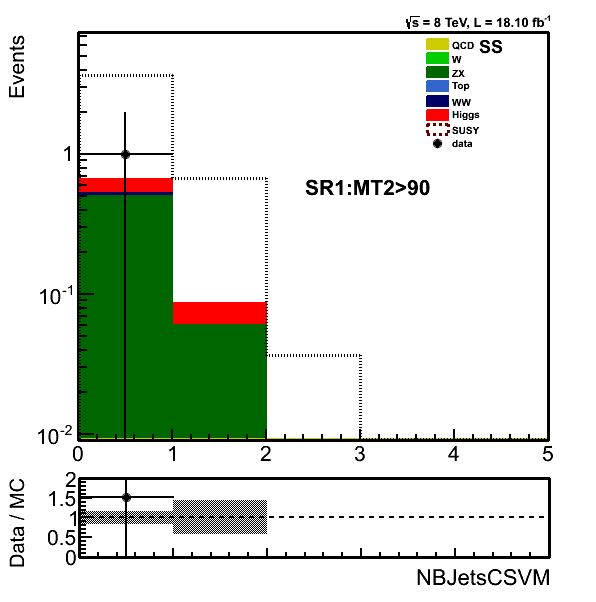
\includegraphics[angle=0,scale=0.35]{TauTauFigs/SR1NBJetsCSVM.png}
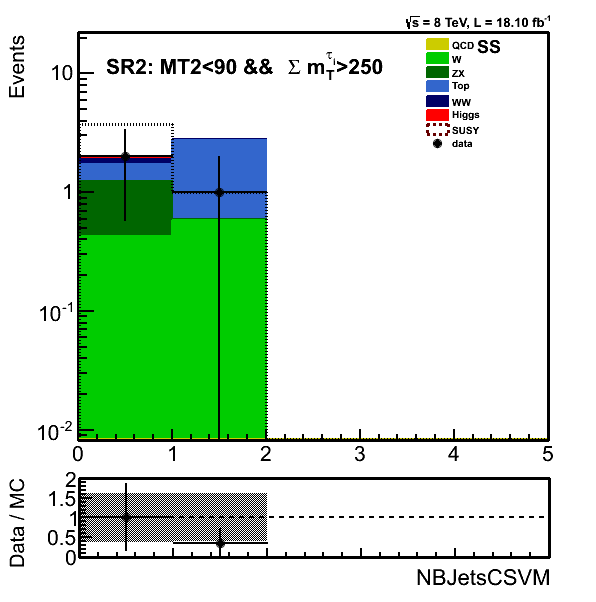
\includegraphics[angle=0,scale=0.35]{TauTauFigs/SR2NBJetsCSVM.png} \\
\caption{The multiplicity of the bjets tagged by CSVM algorithm in the \binone (\bintwo) is shown in left (right).}
\label{fig:nbjets}
\end{figure}
